\documentclass{article}

\title{MATH242 HW3}
\author{Zhangir Azerbayev}
\date{Spring 2022}

% stolen from https://www.cs.cmu.edu/~15131/f17/topics/latex/
\usepackage{amsmath, amsfonts, amsthm, amssymb}  % Some math symbols
\usepackage{mathtools} % defines \coloneqq
\usepackage{enumerate}
\usepackage{fullpage}

\usepackage[x11names, rgb]{xcolor}
\usepackage{tikz}
\usepackage{graphicx}

\usepackage{algorithm}
\usepackage{algpseudocode}

\setlength{\parindent}{0pt}
\setlength{\parskip}{5pt plus 1pt}
\pagestyle{empty}

\def\indented#1{\list{}{}\item[]}
\let\indented=\endlist

\newcounter{questionCounter}
\newcounter{partCounter}[questionCounter]

\newenvironment{question}[2][\arabic{questionCounter}]{%
    \addtocounter{questionCounter}{1}%
    \setcounter{partCounter}{0}%
    \vspace{.25in} \hrule \vspace{0.5em}%
        \noindent{\bf #2}%
    \vspace{0.8em} \hrule \vspace{.10in}%
}{}

\renewenvironment{part}[1][\alph{partCounter}]{%
    \addtocounter{partCounter}{1}%
    \vspace{.10in}%
    \begin{indented}%
       {\bf (#1)} %
}{\end{indented}}


\providecommand{\abs}[1]{\left\vert#1\right\vert}
\providecommand{\norm}[1]{\left\Vert#1\right\Vert}
\providecommand{\pnorm}[2]{\left\Vert#1\right\Vert_{L^{#2}}}
\providecommand{\pnormspace}[3]{\left\Vert#1\right\Vert_{L^{#2}(#3)}}
\providecommand{\pqnorm}[3]{\left\Vert#1\right\Vert_{L^{#2,#3}}}
\providecommand{\pqnormspace}[4]{\left\Vert#1\right\VeFrt_{L^{#2,#3}(#4)}}
\providecommand{\lz}[4]{\left\Vert#1\right\Vert_{L^{#2,#3}\log^{#4}{L}}}
\providecommand{\lzspace}[5]{\left\Vert#1\rig\ht\Vert_{L^{#2,#3}\log^{#4}{L}(#5)}}
\providecommand{\wlt}[1]{\pqnorm{#1}{2}{\infty}}
\providecommand{\Rn}[1]{\mathbb{R}^{#1}}
\providecommand{\intrn}[1]{\int_{\Rn{n}}#1 \,dx}
\providecommand{\csubset}{\subset\subset}
\providecommand{\wnorm}[1]{\lvert \mspace{-1.8mu} \lvert
\mspace{-1.8mu} \lvert #1 \rvert \mspace{-1.8mu} \rvert
\mspace{-1.8mu} \rvert_{L^{2,\infty}}}

\providecommand{\br}[1]{\langle #1 \rangle}
\providecommand{\snorm}[2]{\left\Vert#1\right\Vert_{H^{#2}}}
\providecommand{\snormspace}[3]{\left\Vert#1\right\Vert_{H^{#2}({#3})}}
\providecommand{\sd}[1]{\mathcal{D}_{#1}}
\providecommand{\se}[1]{\mathcal{E}_{#1}}
\providecommand{\sdb}[1]{\bar{\mathcal{D}}_{#1}}
\providecommand{\seb}[1]{\bar{\mathcal{E}}_{#1}}
\providecommand{\snorm}[2]{\left\Vert#1\right\Vert_{H^{#2}}}
\providecommand{\snormspace}[3]{\left\Vert#1\right\Vert_{H^{#2}({#3})}}
\providecommand{\ns}[1]{\norm{#1}^2}
\providecommand{\pns}[2]{\norm{#1}^2_{L^{#2}}}
\providecommand{\dbm}[1]{\bar{D}_m^{#1}}
\providecommand{\ip}[2]{\left(#1,#2\right)}
\providecommand{\iph}[3]{\left(#1,#2\right)_{\mathcal{H}^{#3}}}
\providecommand{\hn}[2]{\norm{#1}_{\mathcal{H}^{#2}}}
\providecommand{\carrow}[1]{\overset{#1}\to}

\def\wstar{\overset{*}{\rightharpoonup}}
\def\nab{\nabla}
\def\dt{\partial_t}
\def\hal{\frac{1}{2}}
\def\ep{\varepsilon}
\def\vchi{\text{\large{$\chi$}}}
\def\ls{\lesssim}
\def\p{\partial}
\def\pa{\partial^\alpha}
\def\sg{\mathbb{D}}
\def\db{\bar{D}}
\def\da{\Delta_{\mathcal{A}}}
\def\naba{\nab_{\mathcal{A}}}
\def\diva{\diverge_{\mathcal{A}}}
\def\Sa{S_{\mathcal{A}}}
\def\Hsig{{_0}H^1_\sigma(\Omega)}
\def\H1{{_0}H^1(\Omega)}
\def\iid{\stackrel{\text{IID}}{\sim}}

\def\F{\mathcal{F}}

\def\a{\mathcal{A}}
\def\E{\mathbb{E}}
\def\f{\mathcal{F}_{2N}}
\def\F{\mathbb{F}}
\def\g{\mathcal{G}_{2N}}
\def\h{\mathcal{H}}
\def\i{\mathcal{I}}
\def\il{\i_{\lambda}}
\def\k{\mathcal{K}}
\def\n{\mathcal{N}}
\def\N{\mathbb{N}}
\def\P{\mathbb{P}}
\def\Q{\mathbb{Q}}
\def\R{\mathbb{R}}
\def\C{\mathbb{C}}
\def\w{\mathcal{W}}
\def\x{\mathcal{X}}
\def\y{\mathcal{Y}}
\def\z{\mathcal{Z}}
\def\Z{\mathbb{Z}}
\def\cf{\mathbb{C}(\F)}

%avg integral
\def\Xint#1{\mathchoice
{\XXint\displaystyle\textstyle{#1}}%
{\XXint\textstyle\scriptstyle{#1}}%
{\XXint\scriptstyle\scriptscriptstyle{#1}}%
{\XXint\scriptscriptstyle\scriptscriptstyle{#1}}%
\!\int}
\def\XXint#1#2#3{{\setbox0=\hbox{$#1{#2#3}{\int}$ }
\vcenter{\hbox{$#2#3$ }}\kern-.6\wd0}}
\def\intbar{\Xint-}

%upper and lower ints
\def\uint{\mathchoice%
    {\mkern13mu\overline{\vphantom{\intop}\mkern7mu}\mkern-20mu}%
    {\mkern7mu\overline{\vphantom{\intop}\mkern7mu}\mkern-14mu}%
    {\mkern7mu\overline{\vphantom{\intop}\mkern7mu}\mkern-14mu}%
    {\mkern7mu\overline{\vphantom{\intop}\mkern7mu}\mkern-14mu}%
  \int}
\def\lint{\mkern3mu\underline{\vphantom{\intop}\mkern7mu}\mkern-10mu\int}
\def\gchar{\ensuremath{\mathrel{\mathrm{char}}}}

\def\L{\mathcal{L}}

\DeclareMathOperator{\curl}{curl}
\DeclareMathOperator{\adj}{adj}
\DeclareMathOperator{\tr}{tr}
\DeclareMathOperator{\diverge}{div}
\DeclareMathOperator{\supp}{supp}
\DeclareMathOperator{\dist}{dist}
\DeclareMathOperator{\card}{card}
\DeclareMathOperator{\vol}{vol}
\DeclareMathOperator*{\argmax}{arg\,max}
\DeclareMathOperator*{\argmin}{arg\,min}


\newenvironment{soln}{\paragraph{Solution:}}{\hfill$\square$}

\theoremstyle{definition}
\newtheorem{lem}{Lemma}[section]
\newtheorem{defn}[lem]{Definition}
\newtheorem{cor}[lem]{Corollary}
\newtheorem{prop}[lem]{Proposition}
\newtheorem{thm}[lem]{Theorem}
\newtheorem{remark}[lem]{Remark}
\newtheorem{example}[lem]{Example}

\newtheorem*{prop*}{Proposition}
\newtheorem*{thm*}{Theorem}
\newtheorem*{def*}{Definition}
\newtheorem*{lem*}{Lemma}
\usepackage{pdfpages}


\begin{document}
\maketitle
Using 3 late days. 


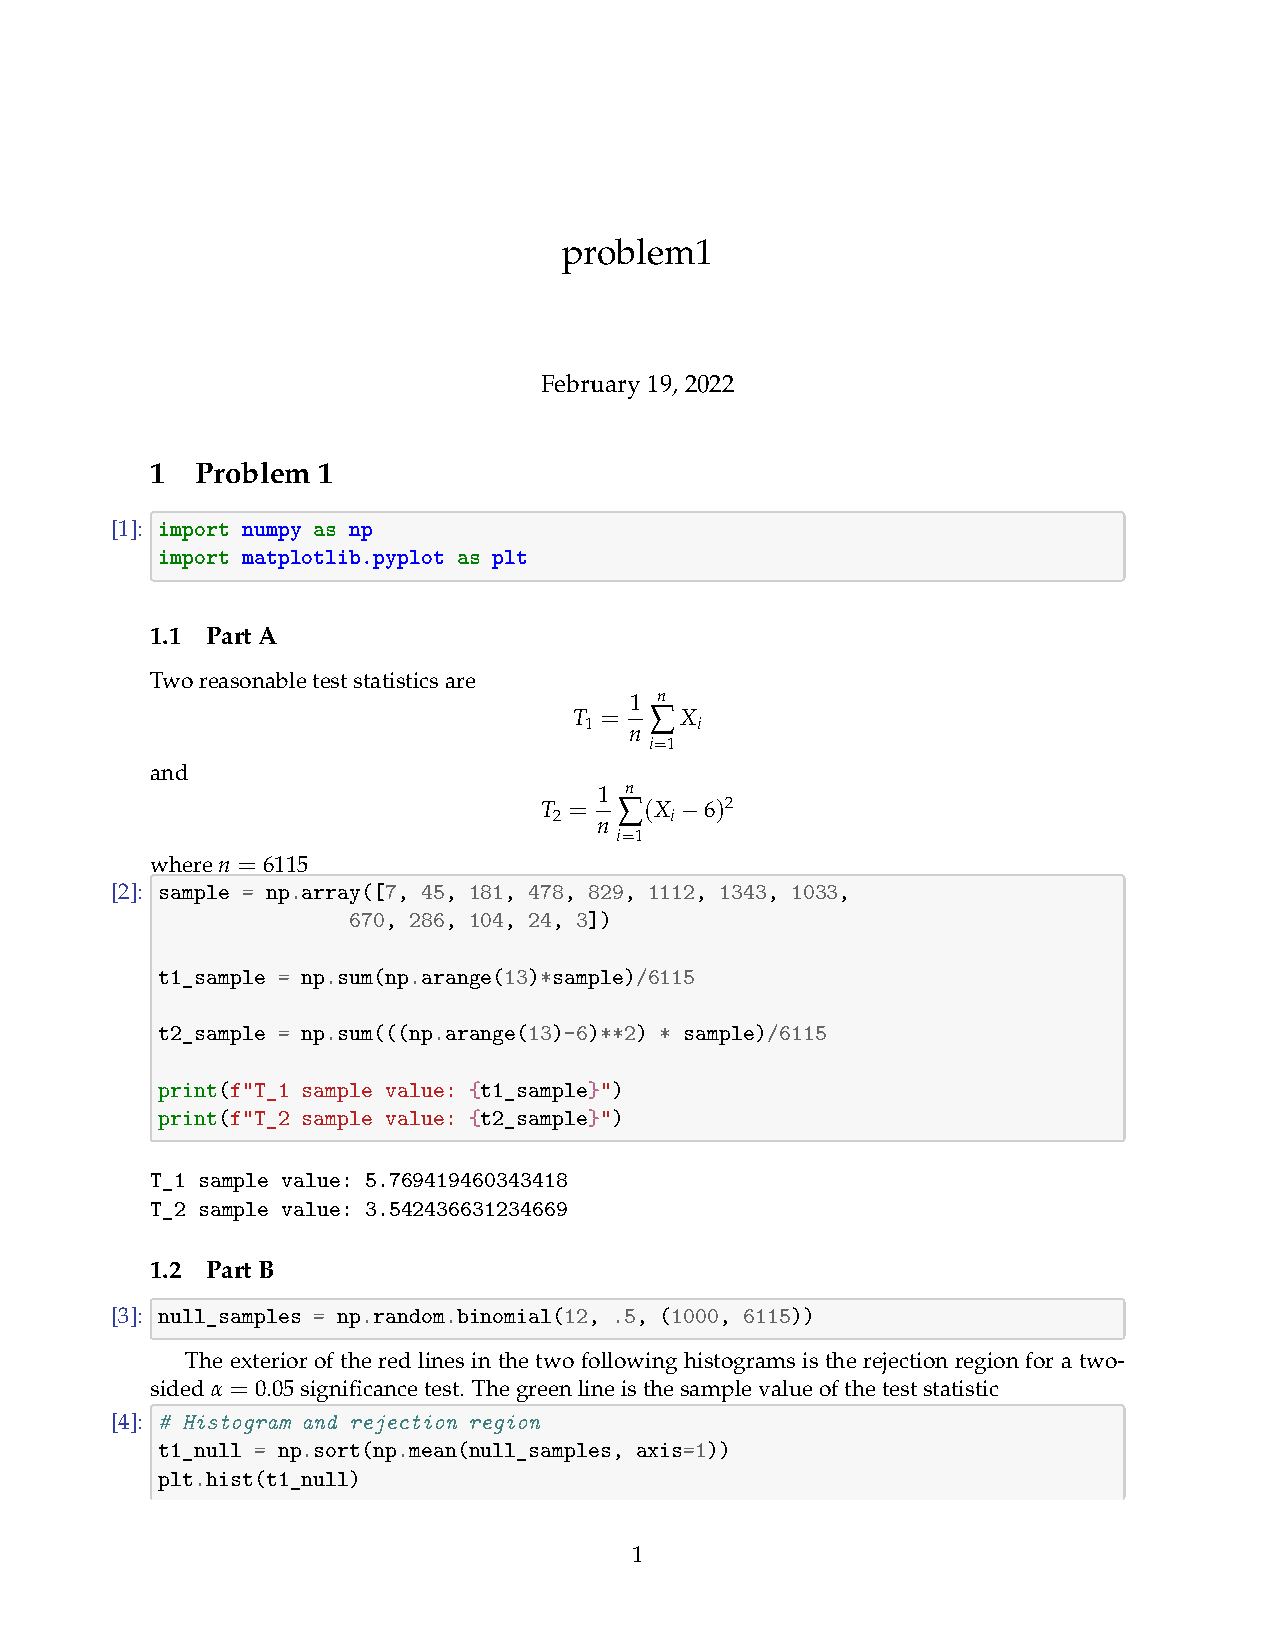
\includepdf[pages=-,pagecommand={},width=\textwidth]{problem1.pdf}

\begin{question}{Problem 2}
    \begin{part}
        Suppose $H_0$. Then $X\sim\mathcal{N}(50, \sigma^2=25)$. The probability of Type I error is $P(|X-50|>10) = P(|z|>2) = 0.05$. 
    \end{part}
    \begin{part}
        Suppose $X\sim \mathrm{Binom}(100, 4/5)$. Then we can approximate $X\sim \mathcal{N}(80, 16)$. Therefore 
        \begin{align*}
            1 - \beta &= P(\text{reject }H_0)\\
                      &= P(|X-50|>10)\\
                      &= P\left(\frac{X-80}{4} > -5 \text{ or } \frac{X-80}{4} < -15/2\right)\\
                      &= P(z > -5 \text{ or } z < -15/2)\\
                      &\approx 1
        \end{align*}
    \end{part}
\end{question}
\begin{question}{Problem 3}
    Since the hypotheses are simple, by the Neyman-Pearson lemma the most powerful test is the likelihood ratio test. Then 
    \begin{align*}
        \alpha &= P_{H_0}(L(X)<c)\\
               &= P_{H_0}\left(\frac{1}{2X} < c\right)\\
               &= P_{H_0}\left(\frac{1}{2c} < X\right)\\
               &= 1 - \frac{1}{2c}. 
    \end{align*}
    Solving for $c$ gives us $c=9/5$. Therefore the power of the test is
    \begin{align*}
        1-\beta &= P_{H_1}(L(X)<c)\\
                &= P_{H_1}\left(\frac{1}{2c} < X\right)\\
                &= \int_{\frac{1}{2c}}^1 2x\mathrm{d}x = 0.19
    \end{align*}
\end{question}
\begin{question}{Problem 4}
    \begin{part}
        We have that 
        \[\prod_{i=1}^nf_0(X_i) = \frac{1}{\sigma_i\sqrt{2\pi}}\prod_{i=1}^ne^{\frac{1}{2}\left(\frac{x}{\sigma_i}\right)^2}. \]
        Therefore
        \begin{align*}
            L(X) &= \left(\frac{\sigma_0}{\sigma_1}\right)^n\exp\left(-\frac{1}{2}\sum_{i=1}^n\left(\frac{X_i}{\sigma_0}\right)^2-\left(\frac{X_i}{\sigma_1}\right)^2\right)\\
                 &= \left(\frac{\sigma_0}{\sigma_1}\right)^n\exp\left(\frac{1}{2\left(\frac{1}{\sigma_1^2}-\frac{1}{\sigma_0^2}\right)}\sum_{i=1}^nX_i^2\right). 
        \end{align*}
        Since $\sigma^2_0<\sigma^2_1$, the likelihood-ratio $L(X)$ is a decreasing function of $\sum_{i=1}^nX_i^2$. Thus setting our test statistic to $T=\sum_{i=1}^nX_i^2$ to perform the likelihood ratio test we need to find $c$ such that 
        \[P_{H_0}(T > c) = \alpha. \]
        Since $\frac{1}{\sigma_0^2}T \sim \chi_n^2$, we can choose $c=\sigma_0^2\chi_n^2(\alpha)$. So our rejection region is $T>\sigma_0^2\chi_n^2(\alpha)$. 
    \end{part}
    \begin{part}
        The distribution of $\frac{1}{\sigma_1^2}T$ under $H_1$ is $\chi_n^2$ (this is equivalent to knowing the distribution of $T$ under $H_1$). We then get 
        \begin{align*}
            1-\beta&= P_{H_1}(T>\sigma_0^2\chi_n^2(\alpha))\\
                   &= P_{H_1}\left(\frac{1}{\sigma_1^2}T>\frac{\sigma_0^2}{\sigma_1^2}\chi_n^2(\alpha)\right)\\
                   &= 1-F\left(\frac{\sigma_0^2}{\sigma_1^2}\chi_n^2(\alpha)\right). 
        \end{align*}
    \end{part}
\end{question}

\end{document}
